\documentclass{ctexart}
\usepackage{amsmath}
\usepackage{geometry}
\usepackage{graphicx}
\usepackage{booktabs}
\usepackage{hyperref}
\usepackage{float}
\title{弦上驻波实验}
\author{陈启钰\,\,2300011447}
\date{\today}
\begin{document}
	\maketitle
	\section{数据及处理}
	\subsection{弦线线密度的测量数据及结果}
	实验中用到的弦线直径为
	\begin{align}
		d_\text{exp}=1.005\mathrm{mm}
	\end{align}
	样品弦线的直径为
	\begin{align}
		d_\text{example}=1.006\mathrm{mm}
	\end{align}
	两者之差
	\begin{align}
		\Delta d=0.001\mathrm{mm}<0.005\mathrm{mm}
	\end{align}
	所以可以将样品弦线的线密度当作实验中所用到的弦的线密度。测得样品弦线的长度、质量分别为
	\begin{align}
		l=78.70\mathrm{cm}, m=4.53\mathrm{g}
	\end{align}
	可得线密度
	\begin{align}
		\mu = \frac{m}{l}=5.76\times 10^{-3}\mathrm{kg/m}
	\end{align}
	\subsection{共振频率与驻波波腹个数的关系}
	由频率公式
	\begin{align}
		f=\frac{N}{2L}\sqrt{\frac{T}{\mu}}
	\end{align}
	给定弦线有效长度$L=60.0\mathrm{cm}$,张力$T=29.403\mathrm{N}$,改变频率使弦线达到不同的共振状态,并计算波速,结果如表\ref{tab:f-N}所示\footnote{这里忽略了倍频现象}。
	\begin{table}[H]
		\begin{center}
			\caption{共振频率$f$与波腹个数$N$的关系}
			\begin{tabular}{ccccccc}
				\toprule
				$N$&$f_\text{theory}/\mathrm{Hz}$&$f_\text{experiment}/\mathrm{Hz}$&$\frac{\Delta f}{f_\text{theory}}/\%$&$v_\text{theory}/\mathrm{m\cdot s^{-1}}$&$v_\text{experiment}/\mathrm{m\cdot s^{-1}}$&$\frac{\Delta v}{v_\text{theory}}/\%$\\
				\midrule
				1&59.6&60.6&1.7&71.5&72.7&1.7\\
				2&119.1&121.3&1.8&71.5&72.9&1.8\\
				3&178.7&183.6&2.7&71.5&73.4&2.8\\
				4&238.2&246.5&3.5&71.5&74.0&3.5\\
				5&297.8&306.7&3.0&71.5&73.6&3.0\\
				\bottomrule
				\label{tab:f-N}
			\end{tabular}
		\end{center}
	\end{table}
	将$f-N$关系作图,得图\ref{fig:f-N}。
	\begin{figure}[H]
		\centering
		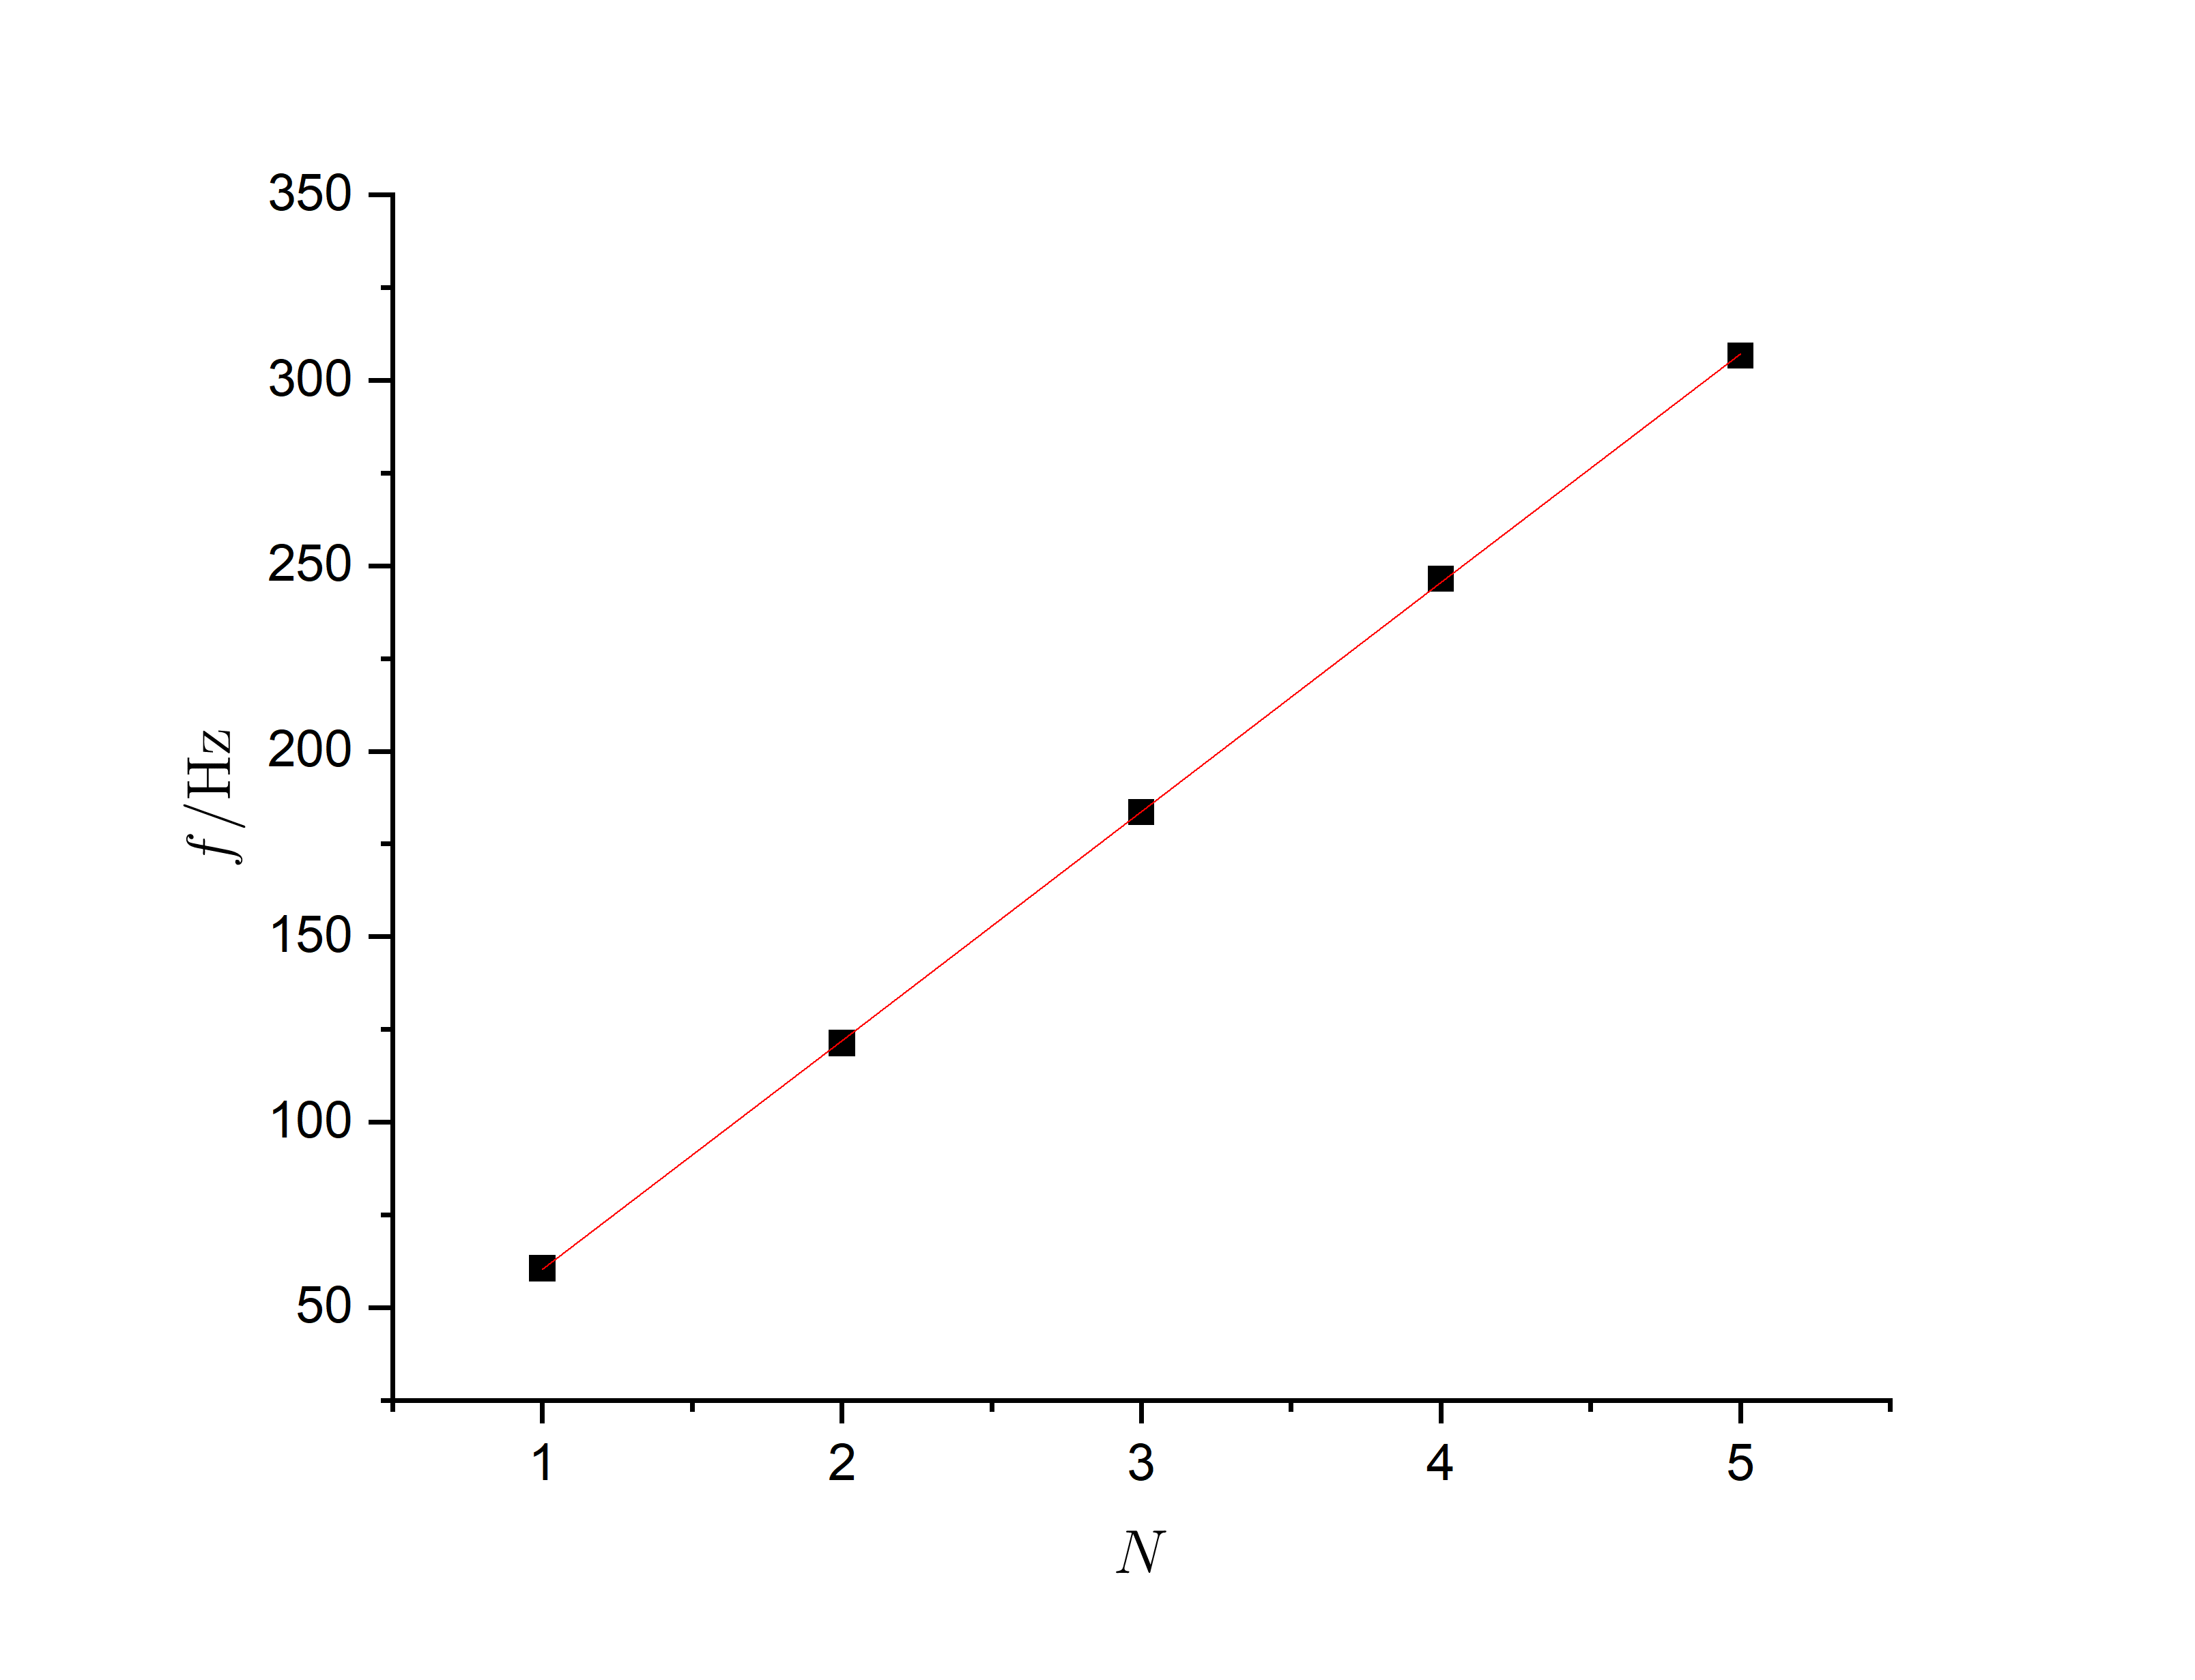
\includegraphics[width=10cm]{fN.png}
		\caption{共振频率$f$-波腹个数$N$关系图}
		\label{fig:f-N}
	\end{figure}
	线性拟合得到
	\begin{align}
		f=61.7N-1.48(\mathrm{Hz}), r=0.99997
	\end{align}
	很好的说明了$f$和$N$之间的线性关系。
	\paragraph{实验现象}
	弦线起振时,可以听到弦线的振动声音变大,弦线有肉眼可见的振动。同时可以看到在调节频率的过程中示波器的CH2通道(连接接收端)的信号幅度变大。随着继续调节频率达到共振状态,可听到声音达到最大,同时肉眼可见的振动最大\footnote{随着波腹个数的增多,振幅越来越不可见,在$N=3$的时候振幅就不太好分辨了},还可以观察到有波节\footnote{即振幅为零的点,实际上看起来很清晰,因为波节不会振动}和波腹。在示波器上可以看到CH2通道振幅最大。
	\paragraph{达到共振的判据}
	达到共振的判据为:①示波器上接收端信号振幅达到最大;②有肉眼可见的波节;③弦线振动声音最大。其中①②为主要判据,③可以方便调节。
	
	同时,在测量共振频率时要保证判据的前后一致性。本实验中,采用的方法是频率从小到大调节,直到信号振幅最大,记录此时的频率值\footnote{一般来说,由于初始条件的不同,从小到大调节和从大到小调节得到的共振频率是不一样的},每次测量完毕后用手按住弦线使其停止振动,然后松开。
	\subsection{共振频率和张力的关系}
	控制弦线有效长度为$L=60.0\mathrm{cm}$,波腹个数$N=1$,改变张力$T$,探究共振频率和张力的关系,得到的结果如表\ref{tab:f-T}所示\footnote{表中对数函数$\ln{x}$的有效数字规则是,改变$x$值的最后一位,则$\ln{x}$也会变化,取其变化的第一位为对数值的最后一位有效数字}。
	\begin{table}[H]
		\begin{center}
			\caption{共振频率$f$与张力$T$的关系}
			\begin{tabular}{cccccc}
				\toprule
				$T/\mathrm{N}$&$f_\text{theory}/\mathrm{Hz}$&$f_\text{experiment}/\mathrm{Hz}$&$\frac{\Delta f}{f_\text{theory}}/\%$&$\ln{f}$&$\ln{T}$\\
				\midrule
				9.801&34.4&35.3&2.6&3.564&2.2825\\
				19.602&48.6&51.0&4.9&3.932&2.9756\\
				29.403&59.6&61.0&2.3&4.111&3.3811\\
				39.204&68.8&70.9&3.1&4.261&3.6688\\
				49.005&76.9&79.0&2.7&4.369&3.8919\\
				\bottomrule
			\end{tabular}
			\label{tab:f-T}
		\end{center}
	\end{table}
	将$\ln{f}$、$\ln{T}$作图,得到图\ref{fig:f-T}。用最小二乘法进行线性拟合,得到
	\begin{align}
		\ln{f}=0.4973\ln{T}+2.436,r=0.99955
	\end{align}
	可见结果与$f^2\propto T$相当接近。
	\begin{figure}[H]
		\centering
		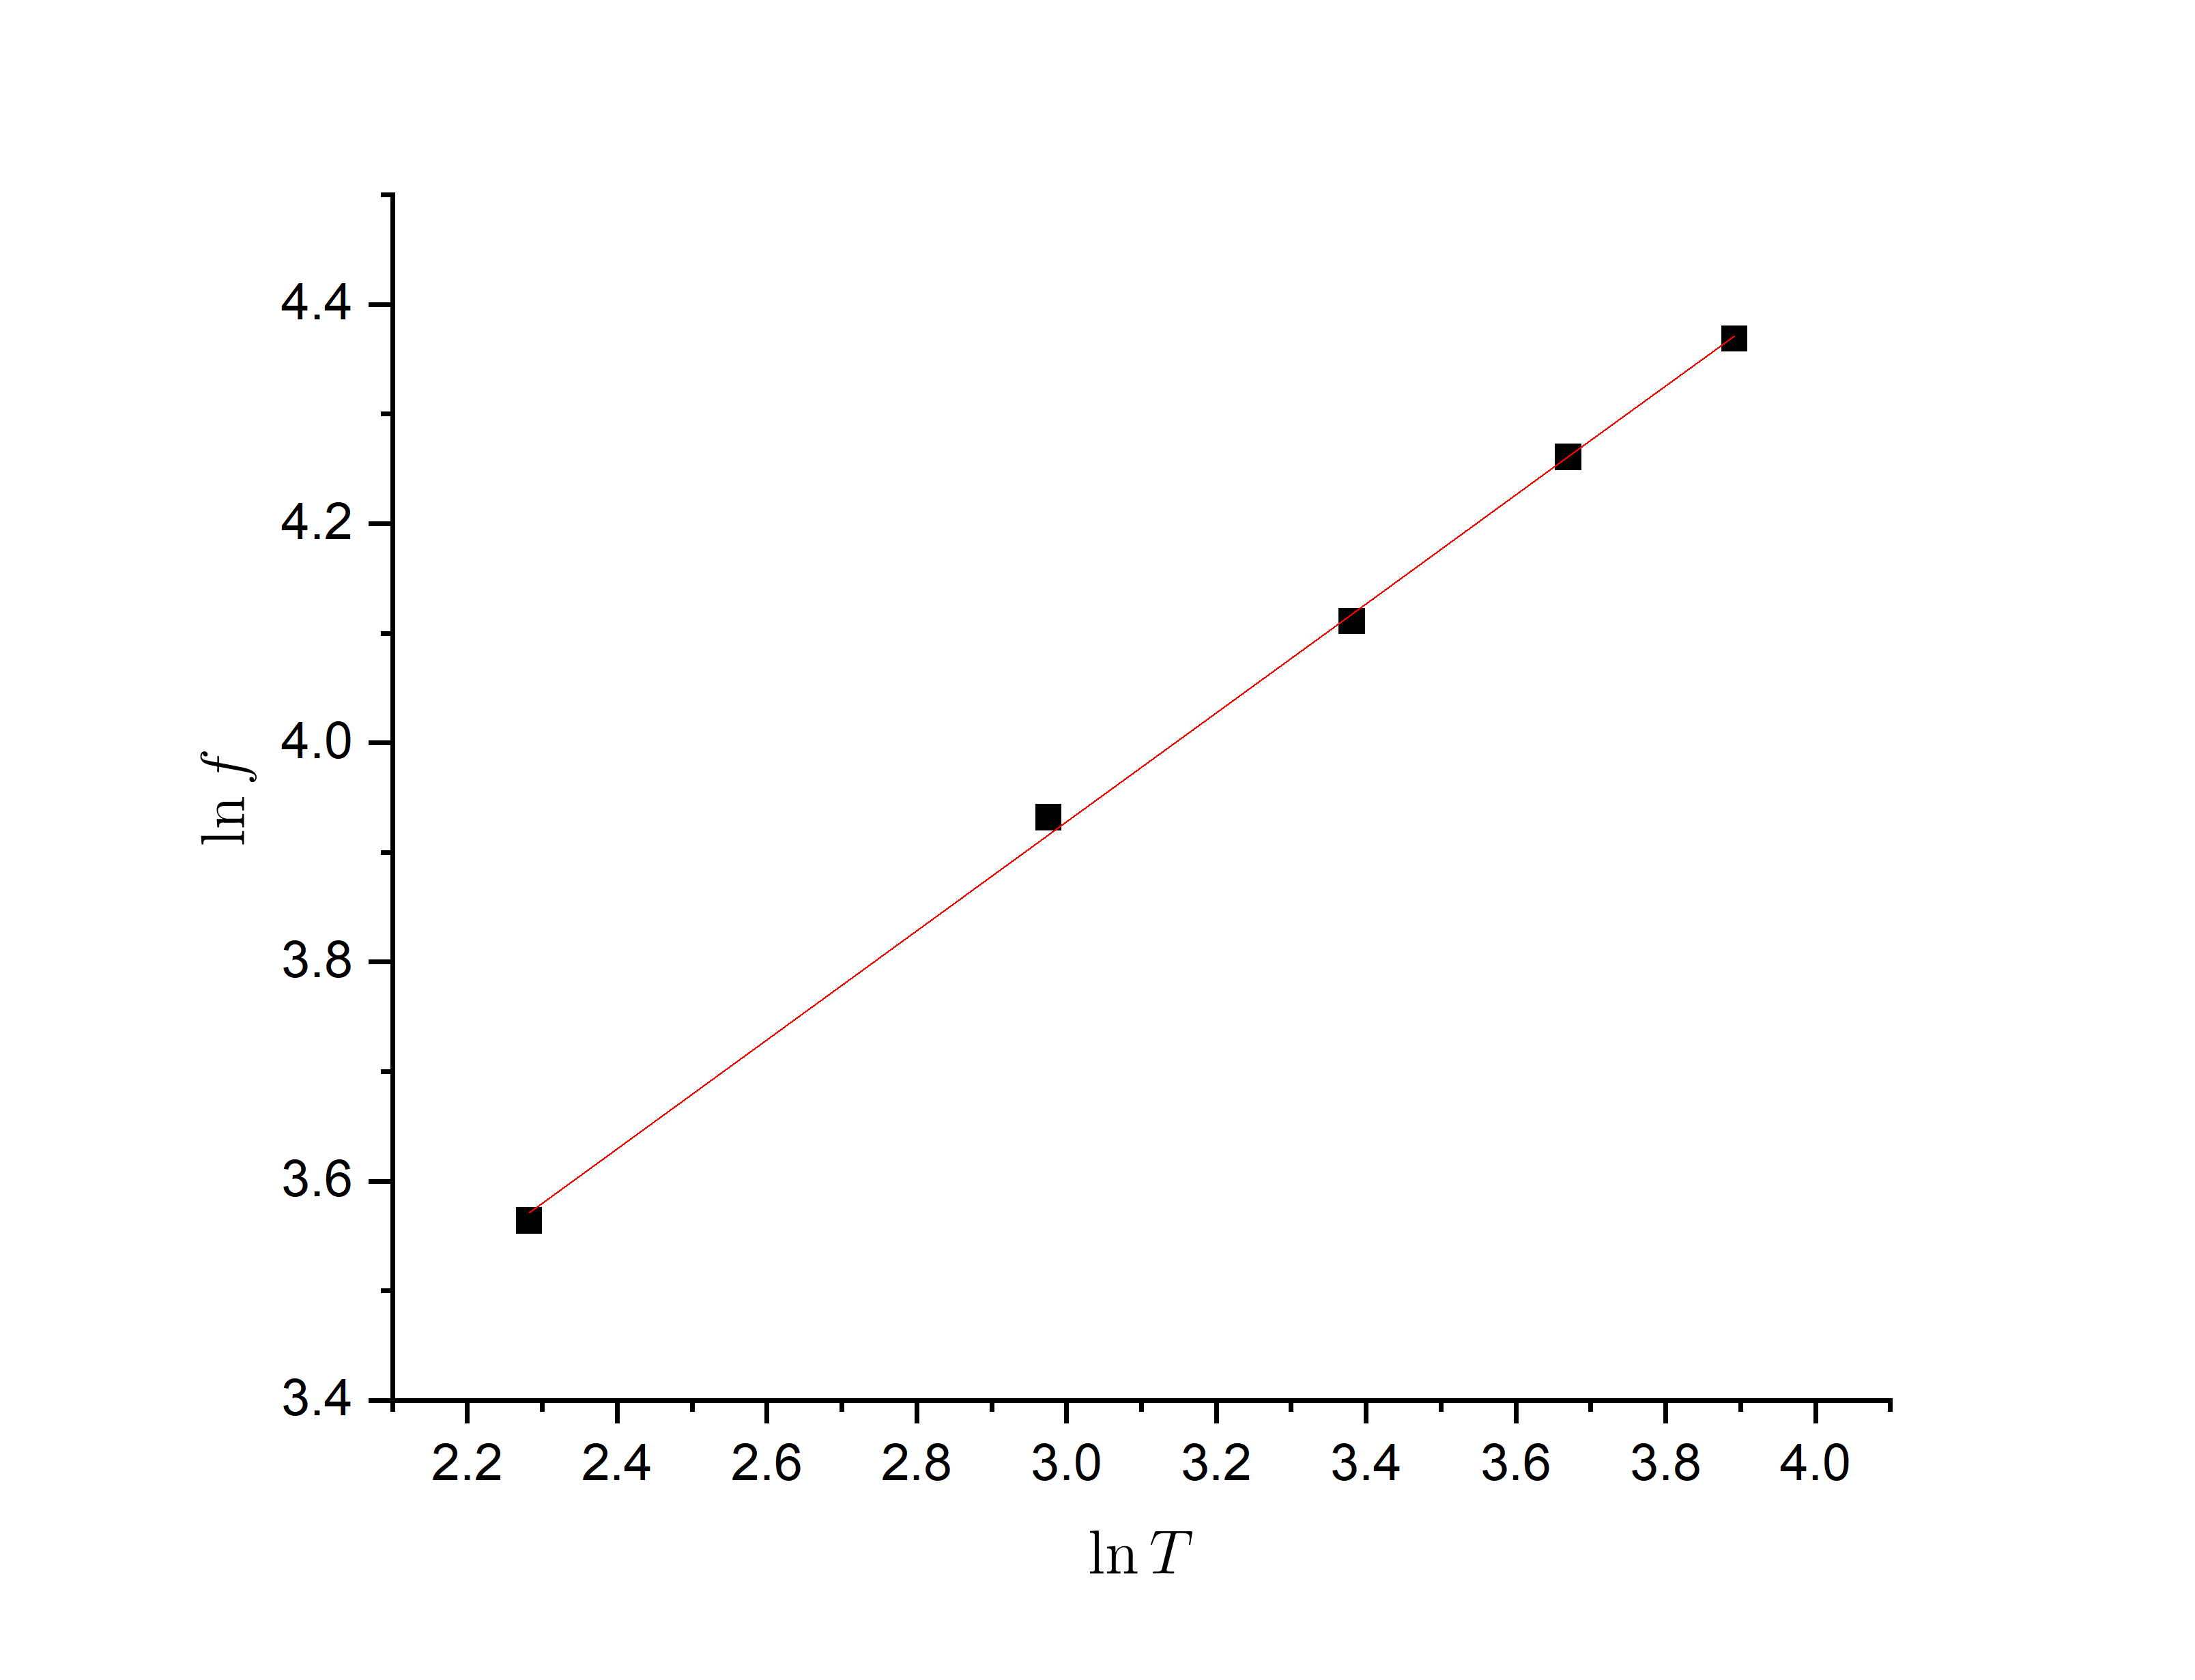
\includegraphics[width=10cm]{fT.png}
		\caption{共振频率$f$-张力$T$关系图}
		\label{fig:f-T}
	\end{figure}
	\subsection{共振频率和弦线有效长度的关系}
	控制波腹个数$N=1$,张力$T=29.403\mathrm{N}$,改变弦线有效长度$L$,探究共振频率和有效长度的关系,得到的结果如表\ref{tab:f-L}所示\footnote{表中$\ln{L}$中的$L$采用的是以$\mathrm{cm}$为单位,这样$\ln{L}$的有效数字会多一些。作为参考,有$\ln{40.1}-\ln{40.0}\approx 2\times10^{-3}$,从而$\ln{40.0}=3.689$有四位有效数字,然而,由于$\ln{0.401}-\ln{0.400}\approx 2\times 10^{-3}$,故$\ln{0.400}=0.916$仅有三位有效数字}。
	\begin{table}[H]
		\begin{center}
			\caption{共振频率$f$与有效长度$L$的关系}
			\begin{tabular}{cccccc}
				\toprule
				$L/\mathrm{cm}$&$f_\text{theory}/\mathrm{Hz}$&$f_\text{experiment}/\mathrm{Hz}$&$\frac{\Delta f}{f_\text{theory}}/\%$&$\ln{f}$&$\ln{L}$\\
				\midrule
				40.0&89.3&91.3&2.2&4.514&3.689\\
				45.0&79.4&81.9&3.1&4.405&3.807\\
				50.0&71.5&73.5&2.8&4.297&3.912\\
				55.0&65.0&67.2&3.4&4.208&4.007\\
				60.0&59.6&61.9&3.9&4.126&4.094\\
				\bottomrule
			\end{tabular}
			\label{tab:f-L}
		\end{center}
	\end{table}
	将$\ln{f}$、$\ln{L}$作图,得到图\ref{fig:f-L}。用最小二乘法进行线性拟合,得到
	\begin{align}
		\ln{f}=-0.9656\ln{L}+8.078,r=0.99987
	\end{align}
	结果与$f\propto L^{-1}$也十分接近。
	\begin{figure}[H]
		\centering
		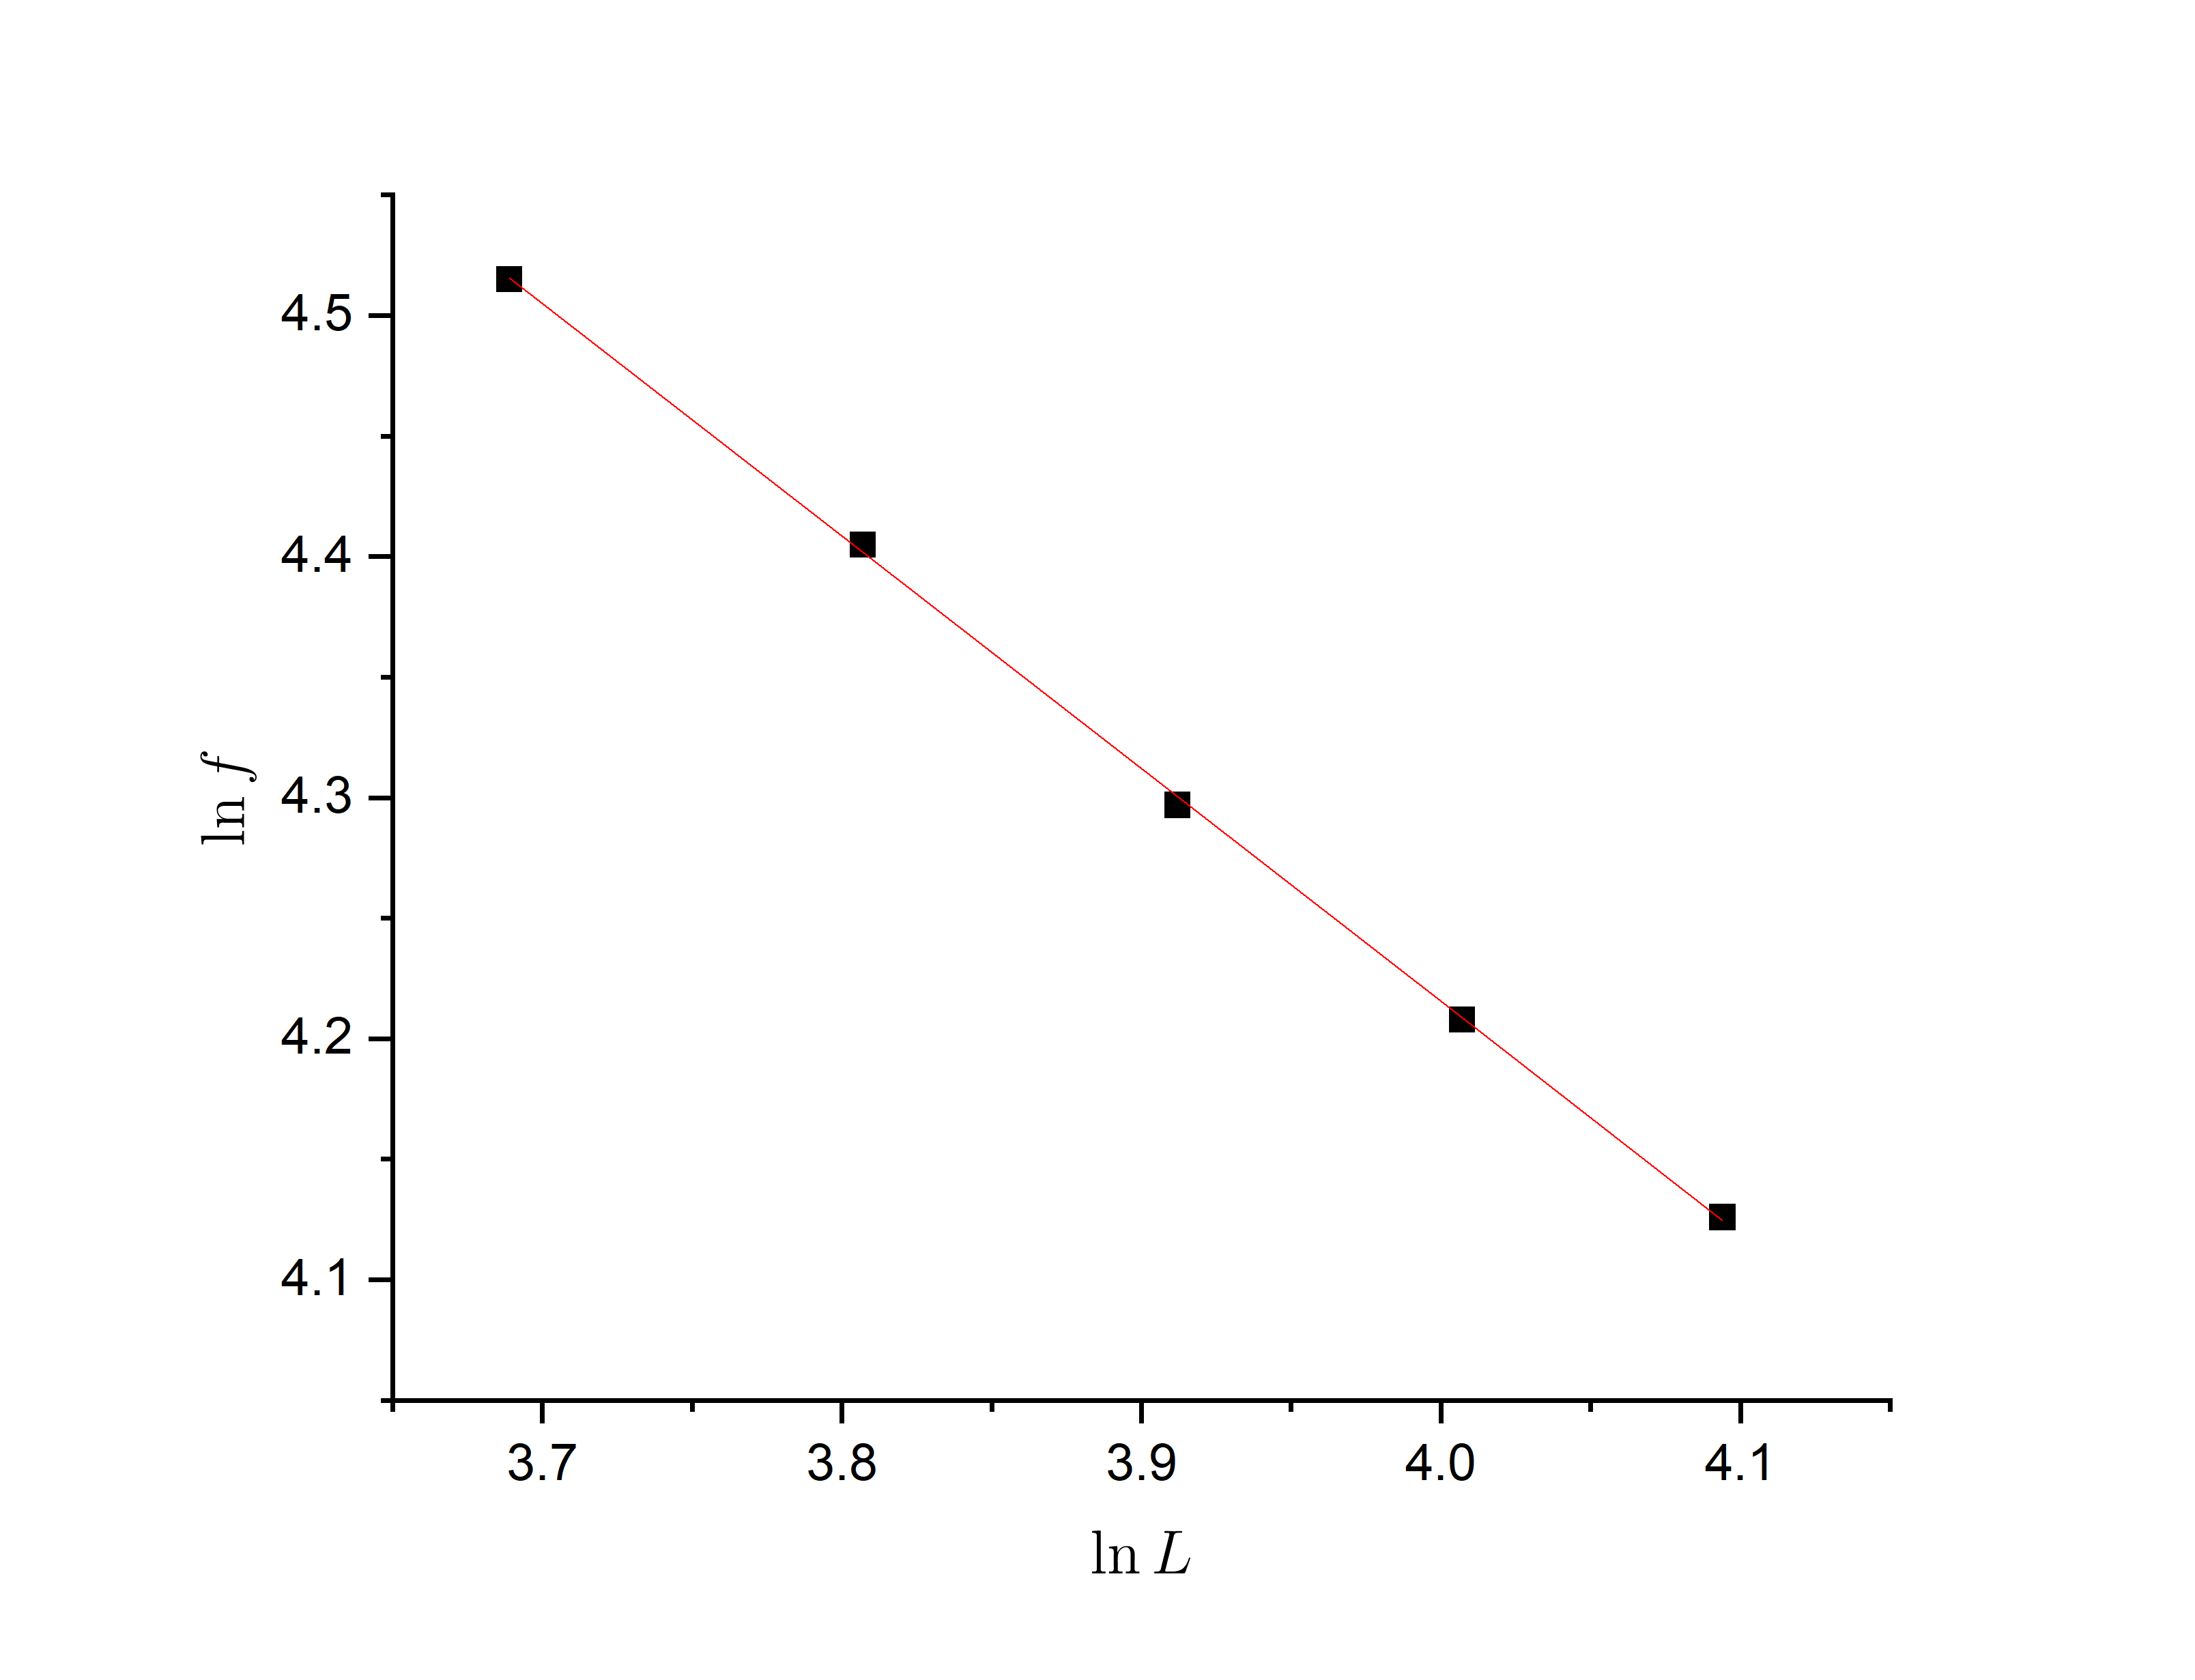
\includegraphics[width=10cm]{fL.png}
		\caption{共振频率$f$-有效长度$L$关系图}
		\label{fig:f-L}
	\end{figure}
	\section{分析与讨论}
	\subsection{主要误差来源}
	\paragraph{测量时的误差}
	在实验过程中,在缓慢调节频率从小变大的过程中,CH2通道信号实际上是不太稳定的,在相当范围内(约$0.5\mathrm{Hz}$),频率的变化并不能直接影响到弦线振动状态的变化(包括振幅,波节等),所以在测量共振频率时会产生一定的误差。另外,由于初始状态的不同和各种非线性效应,以不同的标准测量共振频率也会得到不同的结果,同样会造成误差。
	\paragraph{弦线带来的误差}
	首先,实验用的弦线和样品弦线并不是完全相同的,包括但不限于直径的大小,所以在线密度方面会有一定误差。其次,在振动过程中弦线可能没有张紧,或者弦线有弹性,会造成波动方程不适配,同时产生误差。同时,在实验中注意到张力杠杆和琴弦可能不共线\footnote{琴码上有多处凹槽,而弦线是卡在一个凹槽上的,在杠杆水平的条件下仍有不共线的可能},会造成误差。
	\paragraph{线圈的误差}
	驱动线圈发出的电磁波可能会影响到探测线圈,造成误差。
	
	当然,装置中还有其它的未知非线性效应会对实验结果产生影响,但可能不是误差的主要来源。
	\subsection{倍频现象}
	\paragraph{现象说明}
	在实验过程中,尤其是在基频状态下,会出现倍频效应,即探测到的频率是驱动频率的两倍,但是值得关注的是,倍频效应并不是必然出现的。本实验中,在$L=60.0\mathrm{cm}$、$T=29.403\mathrm{N}$、$N=1$时,调节频率为共振频率,发现弦线共振,只有一个波腹,然后用手按住弦线再释放,弦线以两个波腹振动,且探测到的频率是驱动频率的两倍。使用示波器的FFT功能,发现频谱中有二倍频。
	\paragraph{可能的(模糊的)解释}
	倍频现象本质上是非线性效应,参考\href{https://en.wikipedia.org/wiki/Second-harmonic_generation}{WikiPedia},二次谐波产生(Second-harmonic generation, SHG)是发生在各系统中的最低阶波的非线性相互作用,包括光学、无线电、大气和磁流体动力学系统。
	
	故猜测,磁介质除了最低阶的磁化以外,还可能产生高阶磁化
	\begin{align}
		\mathbf{M}(\omega)=\chi^{(1)}\mathbf{H}(\omega)+\chi^{(2)}\mathbf{H}^2(\omega)
	\end{align}
	不妨设$\mathbf{H}(\omega)=\mathbf{H_0}\mathrm{e}^{\mathrm{i}(\omega t+\phi)}$,则有
	\begin{align}
		\mathbf{M}(\omega)&=\chi^{(1)}\mathbf{H_0}\mathrm{e}^{\mathrm{i}(\omega t+\phi)}+\chi^{(2)}\mathbf{H_0}^2\mathrm{e}^{\mathrm{i}(2\omega t+2\phi)}\\&=\mathbf{M_1}(\omega)+\mathbf{M_2}(2\omega)\notag
	\end{align}
	其中
	\begin{align}
		\mathbf{M_1}&=\chi^{(1)}\mathbf{H_0}\mathrm{e}^{\mathrm{i}(\omega t+\phi)}\\
		\mathbf{M_2}&=\chi^{(2)}\mathbf{H_0}^2\mathrm{e}^{\mathrm{i}(2\omega t+2\phi)}
	\end{align}
	可见,磁化强度$\mathbf{M}$包含二倍频项。同时含有一倍频和二倍频,那么最后得到的驻波就会含有两个波腹(基频状态下)。
	
	那么如何解释某些时候原本只有一个波腹,用手按住并释放后就会有两个波腹呢?这可能与相位匹配有关。若$\chi^{(2)}$包含一个相位,即
	\begin{align}
		\chi^{(2)}=|\chi^{(2)}|\mathrm{e}^{\mathrm{i}\beta}
	\end{align}
	该相位可能存在某些特殊范围使得$\mathbf{M_2}\approx \mathbf{0}$,从而只能看到一个波腹。
	\subsection{小振动条件满足程度对实验结果的影响}
	以波腹个数$N=1$为例,弦线振动的幅度约在$5\mathrm{mm}$,弦线有效长度$60.0\mathrm{cm}$,则最大角约为
	\begin{align}
		\theta_\text{max}=\frac{0.5}{60.0/2}=0.017\mathrm{rad}
	\end{align}
	由理想条件下的波动方程
	\begin{align}
		\frac{\mu}{T}\frac{\partial^2 \xi}{\partial t^2}=\frac{\partial^2 \xi}{\partial x^2}
	\end{align}
	波速
	\begin{align}
		v_0=\sqrt{\frac{T}{\mu}}
	\end{align}
	最大偏差情况下,近似有
	\begin{align}
		\frac{\mu}{T\cos{\theta_\text{max}}}\frac{\partial^2 \xi}{\partial t^2}=\frac{\partial^2 \xi}{\partial x^2}
	\end{align}
	此时的波速
	\begin{align}
		v'=\sqrt{\frac{T \cos{\theta_\text{max}}}{\mu}}
	\end{align}
	两者之比
	\begin{align}
		\frac{v_0}{v'}=\sqrt{\frac{1}{\cos{\theta_\text{max}}}}=1+7\times10^{-5}
	\end{align}
	可见差距极小,甚至小于波速的最后一位有效数字,所以小振动条件在本实验中可以认为是始终满足的。
	\section{原始数据}
	\begin{figure}[H]
		\centering
		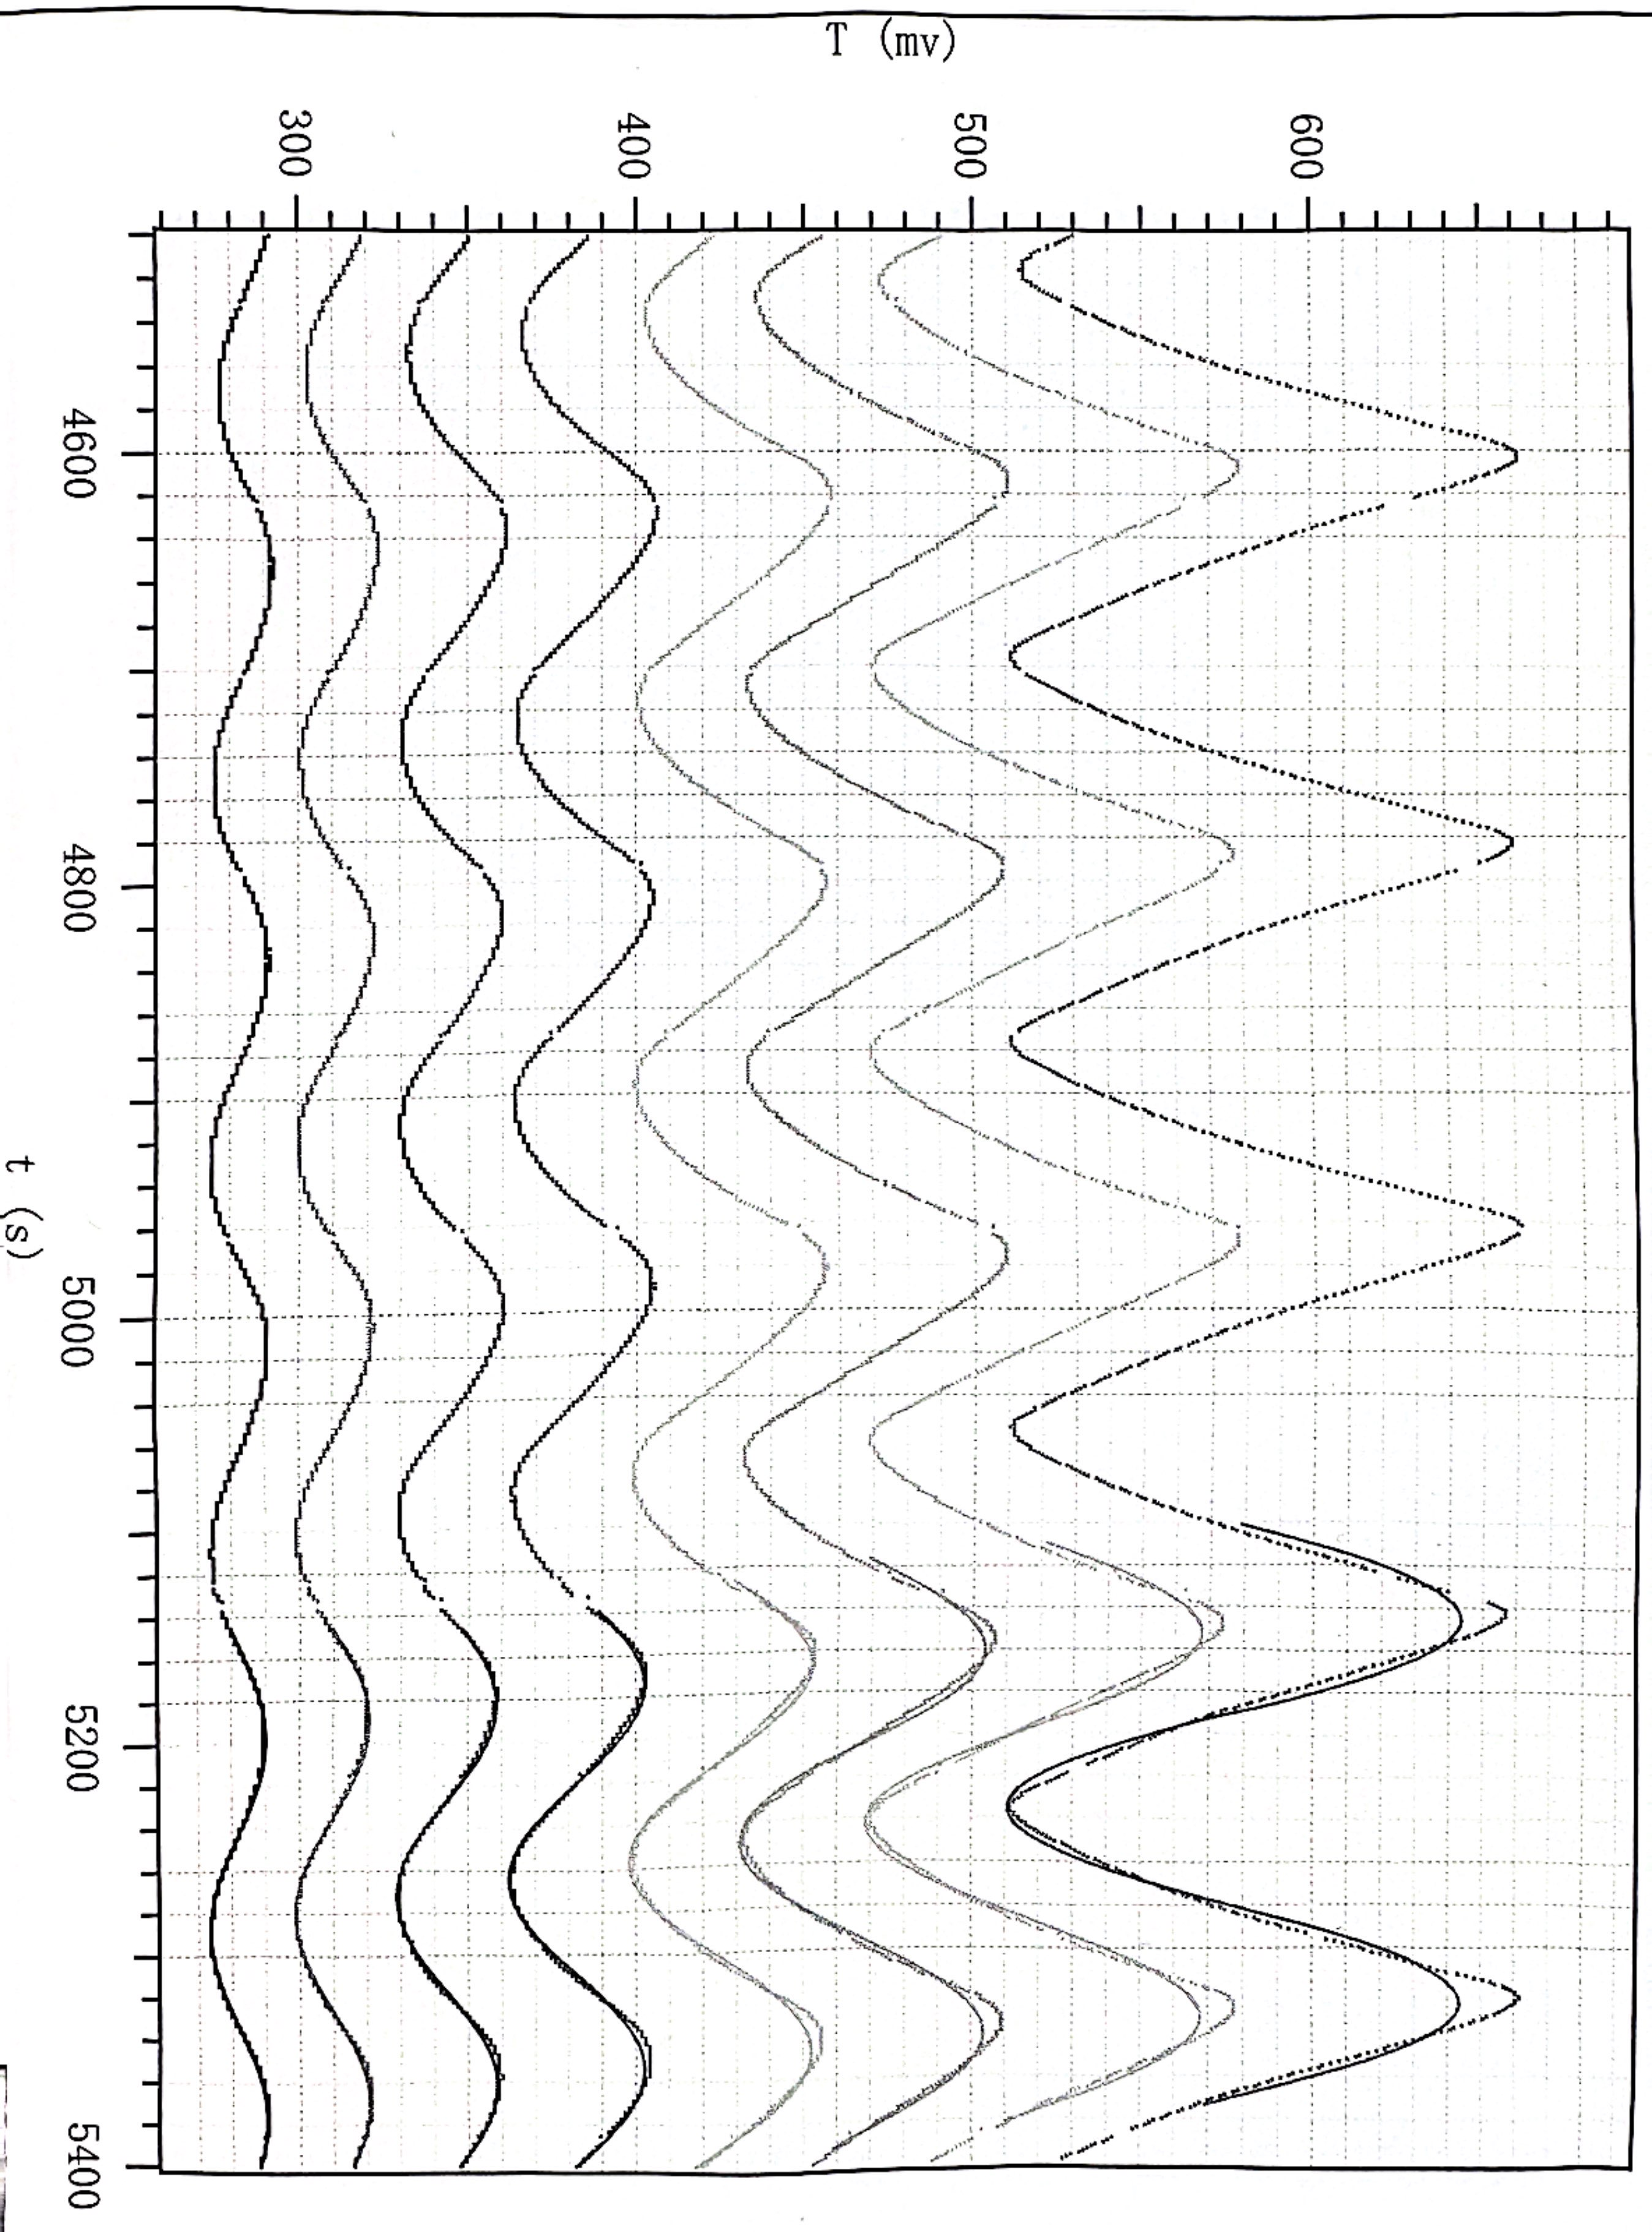
\includegraphics[width=14cm]{data.jpg}
	\end{figure}
\end{document}